% THIS IS SIGPROC-SP.TEX - VERSION 3.1
% WORKS WITH V3.2SP OF ACM_PROC_ARTICLE-SP.CLS
% APRIL 2009
%
% It is an example file showing how to use the 'acm_proc_article-sp.cls' V3.2SP
% LaTeX2e document class file for Conference Proceedings submissions.
% ----------------------------------------------------------------------------------------------------------------
% This .tex file (and associated .cls V3.2SP) *DOES NOT* produce:
%       1) The Permission Statement
%       2) The Conference (location) Info information
%       3) The Copyright Line with ACM data
%       4) Page numbering
% ---------------------------------------------------------------------------------------------------------------
% It is an example which *does* use the .bib file (from which the .bbl file
% is produced).
% REMEMBER HOWEVER: After having produced the .bbl file,
% and prior to final submission,
% you need to 'insert'  your .bbl file into your source .tex file so as to provide
% ONE 'self-contained' source file.
%
% Questions regarding SIGS should be sent to
% Adrienne Griscti ---> griscti@acm.org
%
% Questions/suggestions regarding the guidelines, .tex and .cls files, etc. to
% Gerald Murray ---> murray@hq.acm.org
%
% For tracking purposes - this is V3.1SP - APRIL 2009

\documentclass{acm_proc_article-sp}

\begin{document}

\title{USB in a Microkernelenvironment}
\subtitle{[Extended Abstract]}
%
% You need the command \numberofauthors to handle the 'placement
% and alignment' of the authors beneath the title.
%
% For aesthetic reasons, we recommend 'three authors at a time'
% i.e. three 'name/affiliation blocks' be placed beneath the title.
%
% NOTE: You are NOT restricted in how many 'rows' of
% "name/affiliations" may appear. We just ask that you restrict
% the number of 'columns' to three.
%
% Because of the available 'opening page real-estate'
% we ask you to refrain from putting more than six authors
% (two rows with three columns) beneath the article title.
% More than six makes the first-page appear very cluttered indeed.
%
% Use the \alignauthor commands to handle the names
% and affiliations for an 'aesthetic maximum' of six authors.
% Add names, affiliations, addresses for
% the seventh etc. author(s) as the argument for the
% \additionalauthors command.
% These 'additional authors' will be output/set for you
% without further effort on your part as the last section in
% the body of your article BEFORE References or any Appendices.

\numberofauthors{2} %  in this sample file, there are a *total*
% of EIGHT authors. SIX appear on the 'first-page' (for formatting
% reasons) and the remaining two appear in the \additionalauthors section.
%
\author{
% You can go ahead and credit any number of authors here,
% e.g. one 'row of three' or two rows (consisting of one row of three
% and a second row of one, two or three).
%
% The command \alignauthor (no curly braces needed) should
% precede each author name, affiliation/snail-mail address and
% e-mail address. Additionally, tag each line of
% affiliation/address with \affaddr, and tag the
% e-mail address with \email.
%
% 1st. author
\alignauthor
Daniel Mierswa\\
       \affaddr{RheinMain University of Applied Sciences}\\
       \affaddr{Erlenweg 22}\\
       \affaddr{Taunusstein, Germany}\\
       \email{impulze@impulze.org}
% 2nd. author
\alignauthor
Daniel Tkocz\\
       \affaddr{RheinMain University of Applied Sciences}\\
       \affaddr{Schiffergasse 15}\\
       \affaddr{Wiesbaden, Germany}\\
       \email{daniel.tkocz42@gmail.com}
}
% There's nothing stopping you putting the seventh, eighth, etc.
% author on the opening page (as the 'third row') but we ask,
% for aesthetic reasons that you place these 'additional authors'
% in the \additional authors block, viz.
%\additionalauthors{Additional authors: John Smith (The Th{\o}rv{\"a}ld Group,
%email: {\texttt{jsmith@affiliation.org}}) and Julius P.~Kumquat
%(The Kumquat Consortium, email: {\texttt{jpkumquat@consortium.net}}).}
%\date{30 July 1999}
% Just remember to make sure that the TOTAL number of authors
% is the number that will appear on the first page PLUS the
% number that will appear in the \additionalauthors section.

\maketitle
\begin{abstract}
This paper provides an introduction in using USB in a microkernel.
This paper also contains a small introduction in USB and microkernels for better understanding. Problems that might occur are described and solutions are presented.
%This paper provides a sample of a \LaTeX\ document which conforms to
%the formatting guidelines for ACM SIG Proceedings.
%It complements the document \textit{Author's Guide to Preparing
%ACM SIG Proceedings Using \LaTeX$2_\epsilon$\ and Bib\TeX}. This
%source file has been written with the intention of being
%compiled under \LaTeX$2_\epsilon$\ and BibTeX.

%The developers have tried to include every imaginable sort
%of ``bells and whistles", such as a subtitle, footnotes on
%title, subtitle and authors, as well as in the text, and
%every optional component (e.g. Acknowledgments, Additional
%Authors, Appendices), not to mention examples of
%equations, theorems, tables and figures.

%To make best use of this sample document, run it through \LaTeX\
%and BibTeX, and compare this source code with the printed
%output produced by the dvi file.
\end{abstract}

% A category with the (minimum) three required fields
%\category{H.4}{Information Systems Applications}{Miscellaneous}
%A category including the fourth, optional field follows...
%\category{D.2.8}{Software Engineering}{Metrics}[complexity measures, performance measures]

%\terms{Theory}

\keywords{USB, Microkernel, seL4} % NOT required for Proceedings
\section{Introduction}
In the late late 1990s microkernels became more relevant and were developed more than before. \cite{wiki3}
1996 USB was introduced. \cite{wiki} \cite{wiki2}
This paper is about bringing those two technologies together.\\
Section \ref{sec:usb} is a small and general introduction in USB.
Section \ref{sec:microkernel} describes the structure of a microkernel.
Section \ref{sec:both} describes problems that may occur in a microkernelenvironment using USB and offers solutions.
\section{USB}
\label{sec:usb}
\begin{figure}
\centering

\includegraphics[width=0.2\textwidth]{usblogo.jpg}
\label{fig:usblogo}
\caption{USB 3.0 logo \cite{usborg}}
\end{figure}
USB (Universal Serial Bus) is a serial bus.
With USB it is possible to connect a lot of different types of devices with a host.
Today the most common USB-devices are keyboards and mice. But also external storage, mobilephones and gadgets like a small rocketlauncher can be connected to a host by USB. USB supports hotplugging of USB-devices. That means connecting and disconnecting a USB-device to/from a running host and detecting the USB-device. \cite{wiki} \cite{wiki2}
\subsection{Hardware}
There is a large amount of different USB-connectors (Type A, Type B, Mini A, Mini AB, Mini B, Micro AB, Micro B, Type C). They vary in size, profile, durability, compability and usability.
The used pins used in USB 1.x/2.0 in each of the connectors are nearly the same. \cite{wiki} \cite{wiki2} \cite{usborg}

\begin{table}
\centering
\caption{USB 1.x/2.0 standard pinout \cite{wiki}}
\begin{tabular}{|l|l|l|l|} \hline
Pin & Name & Wire color & Description\\ \hline
1 & $V_{BUS}$ & Red (or orange) & + 5 V\\ \hline
2 & D- & White (or gold) & Data-\\ \hline
3 & D+ & Green & Data+\\ \hline
4 & GND & Black (or blue) & Ground\\ \hline
\end{tabular}
\end{table}

\begin{table}
\centering
\caption{USB 1.x/2.0 mini/micro pinout \cite{wiki}}
\begin{tabular}{|l|l|l|l|} \hline
Pin & Name & Wire color & Description\\ \hline
1 & $V_{BUS}$ & Red & + 5 V\\ \hline
2 & D- & White & Data-\\ \hline
3 & D+ & Green & Data+\\ \hline
4 & ID &  & Detect which connector is connected\\ \hline
5 & GND & Black & Ground\\ \hline
\end{tabular}
\end{table}

Only USB 3.x varies a lot. But some USB 3.0 connectors are backwardcompatible.
$V_{BUS}$ and GND supply the connected device with power varing from specification from 0.5 A to 3 A at 5 V in general. The wires in a USB-cable are twisted to reduce noise. The communication in USB 1.x/2.0 is half-duplex, USB 3.x is full-duplex.
Depending on USB-version the datarate is 1.5 Mbit/s up to 10 Gbit/s. USB 2.0 has a datarate of 480 Mbit/s. \cite{wiki} \cite{wiki2} \cite{usborg} \cite{beyond}

\subsection{Software} %http://www.beyondlogic.org/usbnutshell/usb1.shtml
\subsubsection{Device Descriptor} %http://www.usb.org/developers
The device descriptor specify a couple of informations about a device.
All informations can be printed on the console of a linuxsystem by entering \emph{lsusb -v} in the console. The devicedescriptor is only one descriptor from a small group. There exists the configurationdescriptor -- which describes how much power the device needs, which powermode is used (sleep, selfpowered, etc.), etc. -- , the endpointdescriptor -- described later -- , the interfaceendpoint -- which bundles a group of endpointdesciptors -- and stringdescriptors -- which contain a single string instead of hex-numbers. \cite{beyond}
\paragraph{USB Version}
The devicedescriptor specify the used USB-version. By manipulating this field in the devicedescriptor, a USB 2.0 device can connect to a host as USB 1.1-device. \cite{beyond}
\paragraph{Device Class}
To specify the functionality of a device class codes are used. They are communicated to the host to determine if the device is supported and if so decide which driver should be used for it. For example a device identifiying itself with the classcode $0E_h$ should be treated as a webcam providing a videosignal. In compare to that a device sending $03_h$ should be treated as a human-interface-device (keyboard, mouse, etc.).
If no devicespecific driver exists, in general a generic driver will try to control the device. If the manufacturer thinks none of the deviceclasses matches his needs, the manufacturer can decide to use a vendor specific class: $FF_h$. This might be a good idea for a USB-rocketlauncher. \cite{beyond} \cite{usborg}
\paragraph{Device SubClass}
The subclass specifies more detailed than the device class what the device is. \cite{beyond} \cite{usborg}
\paragraph{Device Protocol}
The protocol field defines a protocol which should be used to communicate with it. \cite{beyond} \cite{usborg}
\paragraph{IDs \& Numbers}
The devicedescriptor contains a vendor-id to identify the manufacturer of a device.
To identify the product of a manufacturer, a product-id is used. To specify the hardwareconfiguration furthermore a device-release-number and a serial number can be specified. \cite{beyond} \cite{usborg}

\subsubsection{Endpoints}
Endpoints are used for communication. Each communication is directed to a specific endpoint. A device/host might have multiple endpoints for different purposes. There are four different types of endpoints. The integrity of a transfer is secured by a CRC-sum for each Endpoint. To end a transfer, each mesage needs to be acknowleged except those from interruptendpoints. Endpoints are configured in an endpointdescriptor. In general the communication has three parts: \cite{beyond}
\begin{itemize}
\item Token Packet
\item Data Packet
\item Handshake Packet
\end{itemize}
Tokenpackets specify the direction of the communication relative to the host. IN means, the host receives data from the device, OUT means the host sends data to the device.\\
Datapackets contains the data or if the passive side of the communication is not ready, it can send STALL or do not respond within a few milliseconds. \cite{beyond}
\begin{figure}
\centering
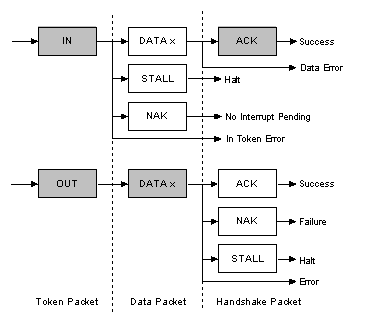
\includegraphics[width=0.4\textwidth]{interrupttransfer.png}
\label{fig:interrupttransfer}
\caption{Protocol of an interrupttransfer \cite{beyond}}
\end{figure}
\paragraph{Control Endpoint}
Controlendpoints are used for controltransfers. With them the device is configured. Every device has a controlendpoint (endpoint zero). \cite{beyond} \cite{wiki2}
\paragraph{Bulk Endpoint}
Bulkendpoints are used for bulktransfers. Bulktransfers are non timecritically, large datatransfers for example a read-/writeoperation on a external storagedevice. \cite{beyond} \cite{wiki2}
\paragraph{Isochronus Endpoint}
Isochronusendpoints are used for isochronustransfers. Isochronustransfers are used if a specific datarate is required. \cite{beyond} \cite{wiki2}
\paragraph{Interrupt Endpoint}
Interruptendpoints are used for interrupttransfers. Other than expected in USB 2.0 and lower this endpoint does not really work with interrupts. Interrupttransfers are polled each x milliseconds. They are often used for human-interface-devices. \cite{beyond} \cite{wiki2}
\subsection{Packets}
For the complete communication packets are used. Each message send from an endpoint and received from an endpoint is based on a simple USB-packet. The packetoverhead is only a few bytes depending on used USB-version. Depending on packettype the packet may contain the following data. \cite{beyond}
\paragraph{Sync}
All packets start with a sync field. The field is used to synchronise the timing of transmitter and receiver. \cite{beyond}
\paragraph{PID}
To specify the content of a packet each sync field of a packet is followed by a PID-field. It contains a 4 bit information about the content. To ensure integrity the PID field contains twice the information to detect biterrors. \cite{beyond}
\paragraph{ADDR}
The ADDR field specifies a divice to communicate with. \cite{beyond}
\paragraph{ENDP}
The ENDP field specifies an endpoint which should receive the packet. Other Endpoints will not notice the packet at all. \cite{beyond}
\paragraph{Data}
The datafield contains up to 1 KB custom data. \cite{beyond}
\paragraph{CRC}
The CRC field contains a CRC sum \emph{only} of the datafield to ensure integrity of the data. \cite{beyond}
\paragraph{EOP}
The EOP-field indicates the end of the package and is everytime the last in field in each package. \cite{beyond}
\section{Microkernel}
\label{sec:microkernel}
A microkernel ($\mu$-kernel) as opposed to a monolothic kernel has fewer code running in
supervisor mode (kernel mode).
\begin{figure}
\centering
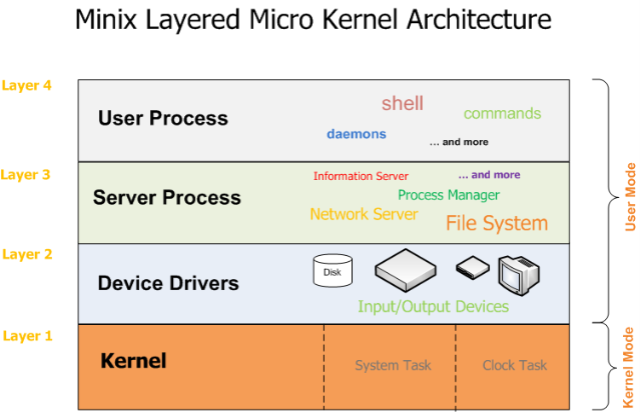
\includegraphics[width=0.4\textwidth]{minixinternalstructure.png}
\label{fig:minixmicarch}
\caption{The microkernel architecture as provided by Minix [minixref]}
\end{figure}
The architecture in of microkernel based operating systems separates basic
hardware functionality from other portions (as seen in Figure \ref{fig:minixmicarch}).
The modularization, if stricly executed, makes it easier for developers to support new
platforms since they only have to port the machine-dependent code for basic hardware functionality.
[black92microkernel]
The code for system specific functionality (services) runs in user mode and as such
is not capable of interfering directly with hardware.
This demonstrates a challenge for driver developers and requires a well-defined kernel API.
Due to the separation and indirection it is believed that microkernels cannot perform as well as
monolithic kernels.
However, most of the performance issues of first generation microkernels were based on poor design
and faulty implementations [p237-liedtke].
Furthermore, device drivers implemented as services on microkernel operating systems can achieve
almost the same performance as monolithic drivers [uldd].

\subsection{Generations}
The idea of a microkernel was introduced in the late 1980s, however at this point Unix [refunix]
was already widely used and adopted.
The concepts of Unix worked good enough around that time and BSD [refbsd] adoption of Unix started
the era of big kernels through adding filesystems and a complete TCP/IP stack. [wiki]
The amount of code in kernels grew fast and with each new code fragment the possibilities of
freezing a system from within a faulty driver implementation increased.
Supporters of microkernel based operating systems argued that user-level implemented TCP/IP drivers
would simply restart the driver and leave the other OS functionality undamaged.
The Mach [refmach] microkernel was developed as a replacement to the mentioned BSD Unix.
It was developed from 1985 to the mid 90s at Carnegie Mellon University and is considered to be
the system that defines the first generation of microkernels.

Mach's external pager [p70liedtke] which manages physical and virtual memory in a way that allows
user-level code to map files and databases into their address space without using the filesystem
driver.
It also llowed the usage of multiple systems simultaenously [p70liedtke].
Another early idea was to implement Interrupt handling via Inter Process Communication (IPC).
IPC is the core component of any microkernel based operating system.
User-level servers can send/receive messages to/from the kernel or other user-level servers
through the kernel.
As one can see the implementation of the communication protocol is a bottleneck and optimization
is necessary to meet the requirements of todays applications.
Analysis of performance problems [p70liedtke] showed that user-kernel-mode switches, address-space
switches and memory penalties also contributed to a bad performance.

In the mid 90s development of new microkernels started.
They were written from scratch rather than evolving from the present monolithic kernels.
One of them was L4 [l4ref].
L4 has three abstraction layers: address spaces, threads and IPC.
Based on tests on a 486-DX5 machine the L4 microkernel RPC was twice as fast as a UNIX system call
and 20 times faster than first generation IPC [p70liedtke].
The address space concept removed another limitation of first generation microkernels.
Basically you were allowed to recursively construct address spaces outside the kernel.
Memory management concepts used in the L4 kernel interface were an extension of the external
pager mechanisms presented in Mach kernels.

\section{USB in Microkernels}
\label{sec:both}
Earlier we presented the basic architecture of USB and how communication works on the serial bus.
In the previous chapter we've seen that microkernels are capable of accessing shared resources
(e.g. a bus) through APIs.
The obvious simple approach to support USB in a microkernel based operating system would be to provide
a service for the interaction with the Host Controller (HC) and let USB device drivers use the HC service.
If another USB device driver uses the HC service the URB coming from this device driver would be
blocked or queued.
This approach would work in a simple 1-to-1 relation when an operating system would just interact
with one USB device.
In real world scenarios however we often face situations where one application (client) uses one or more
devices (interfacing with one or more device drivers), several applications use one or more devices or
devices communicating with each other (data transfer between mass-storage devices).
A simmple ''blocking'' approach does not suffice and another component has to be provided to create a working
environment for USB device drivers.
It has to
\begin{itemize}
\item create URBs based on certain scheduling parameters to avoid blocking
\item fragment data so devices can be polled during huge data transfers
\item prevent unauthorized bus access by other drivers
\end{itemize}
In this paper we try to present a separated USB service which will encapsulate this functionality.

\section{USB service}
We'll look at the Linux USB driver architecture to get an understanding of how to separate concerns
in the handling of the USB protocol and introduce terms we'll be using when describing the design
of the USB service.
\begin{figure}
\centering
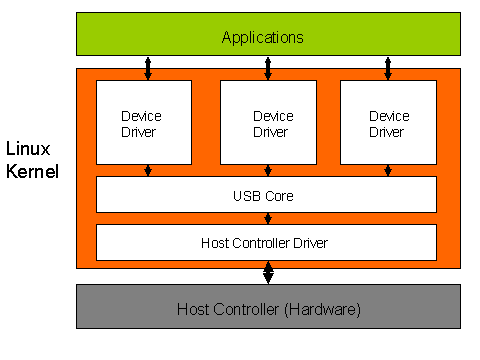
\includegraphics[width=0.4\textwidth]{usblinux.png}
\label{fig:usblinux}
\caption{Main components of the Linux USB driver}
\end{figure}
Figure \ref{fig:usblinux} shows how the operating system USB functionality can be split up into
major components.
The 3 components are:
\begin{itemize}
\item Driver for the Host Controller
\item USBCore support library
\item Drivers for USB devices
\end{itemize}
The Host Controller is the physical component which provides raw hardware access to devices.
The USBCore library is used to abstract functionality of the Host Controller without knowing
the details of the platform like handling interrupts, memory access and configuration.
For the device drivers an interface is provided to manage memory and transfer data.
In addition it provides the USB Request Block (URB) for the specific implementation and ways
to communicate them.
Specific drivers for USB devices can use this library to access hardware and manage data flow.

An USB service would have to implement the USBCore functionality so that specific userspace
USB drivers can be implemented without wrestling with too many problems.
If we consider the 3 functionalities to provide a working USB environment we'll see the 2
main problems: deciding which URBs to send and authorize access.
Not providing a solution to eEither one of those problems could result in data loss,
data corruption or even broken hardware.
We can solve those problems by providing a queue for each driver which will hold the URBs
for this driver and capability based access control.

\subsection{Scheduling}
Looking at URBs in a queue and deciding which URB to pick and send to the bus is called
scheduling.
While there are scheduling algorithms in hardware which can even be configured [chs-ERSA03.pdf]
we will not consider those in the solution provided since it should be possible to implement
the design on any microkernel.
Using scheduling algorithms which decide based on the priority of tasks, such as Fixed priority
preemptive scheduling are not very helpful in this scenario.
Every device driver should be handled equally and thus have the same priority.
If a system is statically configured and/or embedded one could argue that the priorities of
the system are known (e.g. URBs from human interaction devices have a higher priority than
mass storage URBs).
Since the execution time of the operation (transmitting an URB over the bus) should not change
algorithms such as Shortest job first (SJF) are not looked at in this solution.
If the URBs would be scheduled with a First in first out (FIFO) scheduler a faulty driver
or a long operation could block all other drivers from accessing the bus.
Instead the service will have a round-robin approach and will check if any device has URBs
ready to be transmitted.
The device drivers can each schedule their own work.
A mechanism is provided by the server to create a queue in the address space of the server.
This results in IPC between the server and device driver for every URB that is created by
the driver.
Another solution would be the isolation of the URB queue in the address space of the device
driver.
That way would result in an IPC even if the device driver has nothing to transmit as of the
time the server checks if there are URBs ready.

\subsection{Access control}
TODO

\subsection{Design}
TODO

\section{Conclusions}
While designing the USB server it seemed the problems to be
solved are not specific to the domain of microkernels.
The solution presented in this paper designs a single task
that is responsible to grant access and manage data flow
of USB request blocks.
Therefore even the Linux device drivers can be ported
to microkernels by sending the URBs to the server and not to
the Linux kernel itself.
The usb server considers all device drivers and URBs to have
an equal priority which is not really real world applicable.
Future work should provide a parameter to the scheduling system
which gives the server a hint which URB queues to check
more often.
This would result in a scheduler that's no longer completly
fair but which may be better suited for realtime systems or
systems with lots of user interaction (Keyboards, etc.).

\section{Acknowledgments}
We'd like to thank Daniel Ernst and Matthias Jurisch
of Hochschule RheinMain for their design proposal [ref]
which originated from the same ideas we have.
Besides very few specifics our approach is identical.

%
% The following two commands are all you need in the
% initial runs of your .tex file to
% produce the bibliography for the citations in your paper.
\bibliographystyle{abbrv}
\bibliography{sigproc-sp}
%\bibliography{sigproc}  % sigproc.bib is the name of the Bibliography in this case
% You must have a proper ".bib" file
%  and remember to run:
% latex bibtex latex latex
% to resolve all references
%
% ACM needs 'a single self-contained file'!
%
%APPENDICES are optional
%\balancecolumns
\appendix
%Appendix A
\section{Headings in Appendices}
The rules about hierarchical headings discussed above for
the body of the article are different in the appendices.
In the \textbf{appendix} environment, the command
\textbf{section} is used to
indicate the start of each Appendix, with alphabetic order
designation (i.e. the first is A, the second B, etc.) and
a title (if you include one).  So, if you need
hierarchical structure
\textit{within} an Appendix, start with \textbf{subsection} as the
highest level. Here is an outline of the body of this
document in Appendix-appropriate form:
\subsection{Introduction}
\subsection{The Body of the Paper}
\subsubsection{Type Changes and  Special Characters}
\subsubsection{Math Equations}
\paragraph{Inline (In-text) Equations}
\paragraph{Display Equations}
\subsubsection{Citations}
\subsubsection{Tables}
\subsubsection{Figures}
\subsubsection{Theorem-like Constructs}
\subsubsection*{A Caveat for the \TeX\ Expert}
\subsection{Conclusions}
\subsection{Acknowledgments}
\subsection{Additional Authors}
This section is inserted by \LaTeX; you do not insert it.
You just add the names and information in the
\texttt{{\char'134}additionalauthors} command at the start
of the document.
\subsection{References}
Generated by bibtex from your ~.bib file.  Run latex,
then bibtex, then latex twice (to resolve references)
to create the ~.bbl file.  Insert that ~.bbl file into
the .tex source file and comment out
the command \texttt{{\char'134}thebibliography}.
% This next section command marks the start of
% Appendix B, and does not continue the present hierarchy
\section{More Help for the Hardy}
The acm\_proc\_article-sp document class file itself is chock-full of succinct
and helpful comments.  If you consider yourself a moderately
experienced to expert user of \LaTeX, you may find reading
it useful but please remember not to change it.
\balancecolumns
% That's all folks!
\end{document}
